\documentclass[11pt]{article}
\usepackage[margin=1in]{geometry}
\usepackage{amsmath,amssymb,booktabs,array,hyperref,graphicx,algorithm,algpseudocode}
\newcommand{\R}{\mathbb{R}}
\title{\textbf{CASPER: \underline{C}old-start \underline{A}nswerability-aware \underline{S}et-encoder \underline{P}reference \underline{E}licitation by \underline{R}econstruction}\\[4pt]\large Paper B (method) --- working draft}
\author{}
\date{June 2026}
\begin{document}
\maketitle

\begin{abstract}
\noindent Building on the calibrated set-encoder instrument of Paper A, we study \emph{how to choose} elicitation questions for a
cold-start conversational recommender. Our central finding is an \emph{answerability} axis: in true cold-start a user
can answer broad \emph{concept} questions (``do you like horror?'') but not fine \emph{item} questions (``did you like
\emph{this} film?''), having seen almost none of the catalogue---so coarse-but-answerable concepts beat
fine-but-unanswerable items by a wide margin (a $5{:}1$ answer rate; tail NDCG collapses to the no-ask floor when the
same selector is pointed at items). We then learn a policy over the answerable action type that beats the strongest
heuristic (divisiveness) on the long tail and on \emph{every} belief-quality axis (tail NDCG, Recall, MRR,
belief-cosine), while tying the popularity-saturated full metric. The winning recipe is \emph{not} reward maximisation:
from a heuristic-distilled floor, a self-supervised \emph{reconstruction} objective---driving the elicited belief to the
user's own taste vector---is the \emph{only} refinement that helps; REINFORCE and supervised ranking both \emph{degrade}
it, and pretraining is essential. We call this policy \textbf{CASPER-R}. Finally, blind LLM askers show answerability is
a \emph{non-obvious} lesson: model capability predicts answerability-awareness (the strongest avoids items unprompted,
the weakest does not), yet none matches the data-driven policy. CASPER-R is a single policy over a unified item$+$concept
embedding that is simultaneously the recommender.
\end{abstract}

\section{Introduction}\label{sec:intro}
A recommender's hardest moment is the first one. A user who has just arrived has rated nothing, yet the
system must decide what to put in front of them. The standard response to this \emph{cold-start} problem
is \emph{preference elicitation}: ask a short sequence of questions, fold the answers into a user
profile, and only then recommend. The question that has organised two decades of work---and the subject
of this paper---is \emph{what to ask}.

Classical elicitation formulates this as active learning over the catalogue: at each turn pick the
\emph{item} whose rating is most informative, by some surrogate---divisiveness, label entropy, or
expected reduction in reconstruction error~\cite{rashid,golbandi11,elahi16}. This framing has a blind
spot that becomes decisive in genuine cold-start: an item question is only useful if the user can
\emph{answer} it, and a brand-new user has seen almost none of the catalogue. Asking a stranger to rate
a randomly informative film usually yields ``I haven't seen it''---a wasted turn. Rashid et
al.~\cite{rashid} noted two decades ago that a maximally informative item teaches nothing if unseen; we
take this \emph{answerability} constraint as the organising axis of the problem rather than a footnote to
it.

We build on the \emph{calibrated reconstruction instrument} of Paper~A (\S\ref{sec:background}): a single
frozen set-encoder that folds heterogeneous revealed answers---rated items, but also genres and
open-vocabulary \emph{concepts}---into one collaborative-filtering user vector, and which is
simultaneously the recommender. Because this instrument ingests a concept answer (``do you like films
with a \emph{good soundtrack}?'') as readily as an item rating, it lets us pose elicitation over a
\emph{unified} action space of items and concepts, and lets us treat answerability as a tunable
\emph{granularity} choice: coarse-but-answerable concepts versus fine-but-unanswerable items.

This paper reports three results and one method, in increasing order of payoff. \emph{(i)} On the
\emph{discrete} action space of catalogue items, a greedy one-step expected-information-gain (EIG)
selector is the \emph{realizable frontier} \emph{under the noiseless graded/binary answer regime used by simulator
evaluations including ours}---behaviour cloning, oracle distillation, REINFORCE, and
two-step lookahead all match it and none beats it, while a privileged oracle's large headroom is
provably unreachable (\S\ref{sec:discrete}--\ref{sec:gap}). This is the expected outcome for discrete
short horizons: the choice of \emph{action type and criterion} matters enormously (a divisiveness/EIG
selector beats popularity, random, and item-asking by wide margins), but \emph{learning or per-user
adapting} that selection is what adds nothing---localising where a learned policy \emph{can} pay off. \emph{(ii)} The realizable
lever is answerability at \emph{concept} granularity: in realistic cold-start, answerable concepts beat
(mostly unanswerable) item questions by $+50\%$ tail NDCG ($0.140$ vs $0.093$; \S\ref{sec:answerresults}). \emph{(iii)} A
\emph{learned}, answerability-aware policy over the unified item$+$concept pool beats the strongest
heuristic selection of concepts on the long tail---robustly across five seeds---and, given every lever,
it \emph{chooses} to ask zero items, rediscovering the answerability argument as an emergent policy
(\S\ref{sec:learned}--\ref{sec:adapt}). The method that ties these together, and this paper's headline
contribution, is \textbf{CASPER-R}: an answerability-aware elicitation policy over the unified item$+$concept
space, trained not by reward but by self-supervised \emph{reconstruction}.

\paragraph{Contributions, and their lineage.} We are explicit about what is new versus inherited; none of the
ingredients is claimed novel in isolation.
\begin{enumerate}
  \item \emph{(Method, this paper's headline)} \textbf{CASPER-R}: an answerability-aware elicitation policy over the
  \emph{unified} item$+$concept action space of Paper~A's single embedding, trained by a self-supervised
  \emph{reconstruction} objective---driving the elicited belief toward the user's own taste vector---rather than by
  reward. It beats the strongest concept heuristic on the long tail and on every belief-quality axis, and, given items
  and concepts on equal footing, \emph{chooses to ask zero items}, rediscovering the answerability argument as emergent
  behaviour. We credit the unified item$+$attribute action space to ConTS (Li et al.\ 2021, \cite{conts}), which chose a
  \emph{discrete categorical} attribute set by Thompson sampling; our additions are the open-vocabulary \emph{concept}
  granularity, the \emph{reconstruction} training objective (reward and supervised ranking both degrade it), and the
  answerability framing.
  \item \emph{(Result, established)} A \textbf{clarifying negative result}, carefully scoped: on the \emph{discrete} item
  action space, and \emph{under the noiseless graded/binary answer regime used by simulator evaluations including ours},
  greedy one-step EIG is the realizable frontier---behaviour cloning, oracle distillation, REINFORCE, and two-step
  lookahead all match it and none beats it (\S\ref{sec:discrete})---with the oracle's headroom provably unreachable (the
  privileged-imitation gap, Weihs et al.\ \cite{weihs21}; \S\ref{sec:gap}). The claim is emphatically \emph{not} that
  selection is irrelevant---\emph{which} action type and criterion one asks is the dominant lever (the divisiveness
  heuristic beats popularity, random, and items by wide margins, Tables~\ref{tab:answer_cold},~\ref{tab:learned})---but
  that \emph{learning or per-user adapting} that selection adds nothing over the static surrogate in this regime. This is
  the expected outcome for discrete short horizons and localizes where a learned policy \emph{can} pay off:
  \emph{continuous} spaces.
  \item \emph{(Result, established)} The \textbf{answerability lever at concept granularity}. The
  answerability--informativeness tradeoff is foundational---Rashid et al.\ (2002, \cite{rashid}) showed a high-entropy item
  teaches nothing if unseen; Elahi, Ricci \& Rubens (2016) codify acquisition-probability strategies---so we do \emph{not}
  claim it. Our scoped addition: make the lever a \emph{granularity} choice (coarse but answerable \emph{concepts} for fine
  but unanswerable \emph{items}), and show empirically, on Paper A's single unified model, that an answerable-concept policy
  beats item-asking in realistic cold-start (tail NDCG $+50\%$, $0.140$ vs $0.093$).
\end{enumerate}

\section{Background: the calibrated reconstruction instrument}\label{sec:background}
All experiments share one frozen artefact from Paper~A, summarised here because every elicitation result
depends on three of its properties: it is a \emph{set-encoder}, it ingests \emph{heterogeneous} answers,
and it is \emph{calibrated}.

\paragraph{Reconstruction fold-in.} The instrument is an attention set-encoder $\Phi$ mapping a set of
revealed (entity, answer) tokens to a user vector $u=\Phi(\{(\phi_e,a_e)\})\in\R^{D}$ ($D{=}64$), where
$\phi_e$ is the entity embedding and $a_e$ the signed answer. Items embed as their biased-SVD factors
$q_i$; a concept embeds as $E_c$, the centroid of the items carrying that Tag-Genome tag. The
recommender score for item $i$ is $s_i=\mathrm{pop}_i+q_i^\top u$, so eliciting answers and ranking the
catalogue use \emph{the same} embedding---the encoder \emph{is} the recommender. The fold is
order-invariant and defined on any subset, which is precisely what lets a policy ask an arbitrary
\emph{mixture} of items and concepts and read out a fresh profile after every turn.

\paragraph{Geometric answers.} A new user's response is simulated geometrically against their held-out
true-taste vector $u^\star$: an item answer is the taste residual $r_{ui}-\mu-b_i$ when the user has
rated $i$; a concept answer is $\mathrm{sign}(u^{\star\top}E_c-\theta)$, scaled to the population
like/dislike residual---``do your tastes fall on the liked side of this concept?''. An item is
\emph{answerable} only if the user has rated it; a concept only if the user has $\ge 2$ items in it. This
answerability constraint drives every result below.

\paragraph{Calibration, and why it matters here.} Paper~A established that the instrument is
\emph{monotone and no-harm}: folding a truthful answer does not decrease expected held-out quality on
RMSE, Recall@50, or NDCG@10. This makes the elicitation question well-posed---a good question cannot be
``punished'' by a miscalibrated encoder---so we can read a clean information signal off the fold rather
than fighting the representation collapse that defeated earlier signed/contrastive encoders.

\paragraph{Protocol and metrics.} Throughout we simulate true cold-start: the test user starts
\emph{empty}; we ask $T$ questions over the \emph{full catalogue}; we fold each answer; and we measure
held-out NDCG@10 and Recall@50, both full-catalogue and long-tail (the Cremonesi head/tail
split~\cite{cremonesi10}; head ${=}$ the most-popular $33\%$ of likes). Test users are disjoint from
training; for the learned policy the validation users used for model selection are disjoint from the
test users as well (\S\ref{sec:learned}). All ``seed-averaged'' numbers average five held-out user-split
seeds $\{1,2,3,7,11\}$ (a seed randomizes the held-out user split; te$[300{:}]$ denotes the evaluation
cohort within each split).\footnote{On a sixth split (seed $123$) CASPER-R's tail margin over the
fair-entropy heuristic is smallest ($+0.002$) but does not reverse; the per-seed delta is positive on all
six splits.}

\section{Related Work}\label{sec:related}
\paragraph{Preference elicitation and active learning in recommenders.} The cold-start interview has a
long lineage. Rashid et al.~\cite{rashid} introduced ``getting to know you'' strategies and the
entropy/popularity trade-off; their HELF heuristic (harmonic mean of normalised entropy and
log-frequency) is still a standard non-personalised baseline. Golbandi et al.~\cite{golbandi11} build an
adaptive \emph{decision tree} over items with like/dislike/unknown branches, greedily minimising
population reconstruction error---the static-then-adaptive interview we compare against
(GREEDYEXTEND/tree). Elahi, Ricci \& Rubens~\cite{elahi16} survey active learning in collaborative
filtering and codify acquisition-probability strategies that weight informativeness by the chance the
user can answer. Our addition is not the answerability \emph{idea}---foundational here---but making it a
\emph{granularity} lever (concepts vs.\ items) on a single instrument that can ask either, and exhibiting
a learned policy that navigates it.

\paragraph{Conversational recommendation.} A parallel line builds multi-turn agents that alternate asking
\emph{attributes} and recommending \emph{items}: EAR~\cite{ear}, SCPR, and UNICORN~\cite{unicorn}
formalise this as RL or graph reasoning but \emph{split} the action space into separate ``ask-attribute''
and ``recommend-item'' heads. ConTS~\cite{conts} removes the split, placing items and attributes in
\emph{one} unified action space chosen by Thompson sampling---but over a discrete, finite, categorical
attribute set. We inherit ConTS's unified-action insight and push it two ways: the attributes become
\emph{open-vocabulary concepts} in a continuous embedding, and the asker becomes a \emph{learned} policy
rather than a bandit.

\paragraph{Sequential experimental design and RL for elicitation.} Choosing questions to maximise
information is Bayesian optimal experimental design; amortised/deep variants (DAD~\cite{dad}) and
sequential-design RL (Blau et al.~\cite{blau22}, Bakker et al.~\cite{bakker20}) give the sharpest
reference for \emph{when} a learned non-myopic policy beats greedy one-step information gain---empirically
in \emph{continuous} design spaces, not discrete short horizons (\S\ref{sec:discrete}). In recommendation,
NICF~\cite{nicf} casts the cold-start interview as deep value-based RL with a self-attentive history
encoder; we reimplement it on our ruler as the deep-RL baseline. For the action space, Wolpertinger
\cite{wolp} introduced the continuous-proto-action plus nearest-neighbour-snap mechanism for large
discrete action sets, which we adopt to make a continuous policy over the unified item$+$concept
embedding tractable. None of these asks a continuous \emph{mixture} of items and open-vocabulary concepts;
that combination is our method's locus.

\section{The discrete elicitation frontier: greedy information gain is realizable-optimal}\label{sec:discrete}
\paragraph{No policy beats greedy info-gain on items.} With the frozen instrument and \emph{answerable} items, we gave a
learned policy its best shot across four method families---behaviour cloning~\cite{ross11}, oracle distillation
(pointwise MLP and a set-transformer over candidates), REINFORCE fine-tuning, and explicit two-step lookahead
planning---and \emph{every} realizable method only \emph{matches} a deployable greedy one-step expected-information-gain
(EIG) selector; none beats it (all within noise of $0.371$ full / $0.194$ tail NDCG@10), \emph{under the noiseless
graded/binary answer regime used by simulator evaluations including ours}. To be precise about what carries the value:
\emph{which} action type and criterion one selects matters enormously---the EIG/divisiveness heuristic beats popularity,
random, and item-asking by wide margins (Tables~\ref{tab:answer_cold},~\ref{tab:learned})---but \emph{learning or per-user
adapting} that selection is what adds nothing over the static one-step surrogate on discrete items. A \emph{privileged}
oracle that peeks at the held-out targets has large headroom ($0.564/0.395$) but, depending on hidden answers, is not a
realizable method.

\paragraph{This is what the literature predicts for discrete short horizons.} In discrete, short-horizon active
information acquisition, learned non-myopic policies are known to only \emph{match} greedy one-step information gain:
Blau et al.~\cite{blau22} report deep-RL sequential experimental design within $\sim$1\% (inside the standard error)
of a myopic baseline on a discrete task, and Bakker et al.~\cite{bakker20} find a greedy one-step approximation
``nearly on-par'' with a non-myopic policy-gradient policy. The clearest discrete win for RL over the same surrogate's
greedy policy, GSMRL~\cite{gsmrl}, bundles a \emph{generative surrogate} (side information) with dense potential-based~\cite{ng99}
information-gain shaping; the explicit-planning method NOCTA~\cite{nocta} beats greedy but reports its own RL baselines
\emph{underperforming} greedy. Our convergent result---four method families matching greedy---is therefore the
expected outcome, not an artefact.

\subsection{Why distilling the oracle is \emph{worse}, not equal: the privileged-imitation gap}\label{sec:gap}
Distillation matches a teacher only when the teacher is \emph{realizable}---a function of the observable state. EIG is
(its choices depend only on the belief), so distilling EIG recovers EIG. The oracle is \emph{not}: its choice
$c^\star=\arg\max_c \mathrm{NDCG}_{\text{test}}(c)$ depends on the held-out targets. Behaviour cloning a teacher whose
actions depend on information the student cannot see does not recover the teacher's performance; it learns the
state-projection of the oracle's actions---``what kind of item the oracle tends to pick''---which, stripped of the
targets, is a \emph{miscalibrated} criterion: those items were good because they aligned with hidden targets, not
because they are informative. Our set-transformer makes this concrete: it is expressive enough to \emph{reproduce} the
oracle's choices (63\% top-1 agreement), yet executing them without the targets scores \emph{below} greedy EIG
below greedy. This is precisely the privileged-information imitation gap of Weihs et al.~\cite{weihs21}:
cloning a privileged expert can yield a policy arbitrarily worse than a sensible learnable baseline, because the
objective collapses to the expert's action distribution marginalised over the unobserved latent. Hence ``distillation
should at least match'' holds for EIG but \emph{fails} for the oracle---and the oracle's headroom is genuinely
unreachable.

\paragraph{So the lever is the action \emph{type}, not the policy.} If no policy beats greedy on items, the gain must be
in \emph{what} we ask. Paper A's question-type analysis is decisive: items are maximally informative but only $\sim$2\%
answerable in cold start, genres answerable but coarse, and fine \emph{concepts} both answerable ($\sim$57\%) and
near item-level informative. The rest of this paper therefore makes \emph{answerability} the central axis and learns a
policy over the answerable concept space (\textbf{CASPER-R}, \S\ref{sec:learned}). A \emph{second} lever---continuity:
non-myopic RL beats greedy in \emph{continuous} design spaces but only matches it in discrete ones (Blau et
al.~\cite{blau22}; amortised design DAD~\cite{dad})---motivates a continuous, open-vocabulary actor over the unified
item$+$concept space (ConTS~\cite{conts} unified actions $+$ a Wolpertinger~\cite{wolp} continuous snap), which we take
up in Paper~C.

\section{Answerability in realistic cold-start: concepts beat items}\label{sec:answerresults}
We instantiate the answerability argument empirically on the unified instrument (Paper A's concept-aware encoder; ML-1M;
true cold-start: the user starts empty and we ask $T{=}8$ questions over the \emph{full catalogue}; an item question is
answered only if the user has actually seen it, a concept question if the user has $\ge 2$ items in it; held-out NDCG@10
and Recall@50, full and long-tail). Table~\ref{tab:answer_cold} is the core evidence.
\begin{table}[h]\centering\small
\begin{tabular}{l l cc c c}
\toprule
selection criterion & pool & FULL & TAIL & ans & $\cos$\\
 & & NDCG & NDCG & /8 & $(u,u^\star)$\\
\midrule
--- (ask nothing, $q0$) & MostPop & 0.310 & 0.081 & 0 & 0.00\\
\midrule
divisiveness (entropy) & concepts & 0.361 & \textbf{0.140} & 5.2 & 0.64\\
 & items & 0.304 & 0.093 & \textbf{0.5} & 0.16\\
 & items$+$concepts & 0.315 & 0.102 & 0.8 & 0.28\\
\midrule
popularity & concepts & 0.346 & 0.126 & 8.0 & 0.81\\
 & items & 0.331 & 0.100 & 1.9 & 0.45\\
 & items$+$concepts ($50/50$) & 0.352 & 0.128 & 5.1 & 0.80\\
\midrule
\emph{full-profile ceiling} & all known & 0.407 & 0.216 & --- & 1.00\\
\bottomrule
\end{tabular}
\caption{\textbf{Answerability, isolated} (seed-averaged, te$[300{:}]$, $q8$). Holding the selection criterion fixed and
changing only the \emph{pool}: over \emph{concepts} a user answers $5.2/8$ (divisiveness) or $8/8$ (popularity) and NDCG
lifts; point the \emph{same} criterion at \emph{items} and only $0.5$--$1.9/8$ land---divisive/popular items are unseen
in cold-start---so tail NDCG \emph{collapses toward ask-nothing} ($0.093$--$0.100$ vs $0.081$) and the belief barely
forms ($\cos\,0.16$--$0.45$). The mixed pool is dragged down too: the answerability cost of items is not offset by their
fine signal. \emph{Items are fine questions that cannot be answered cold}---the central lever of this paper. (The
answerability axis is foundational, Rashid et al.\ \cite{rashid}; our contribution is the item-vs-concept
\emph{granularity} framing and this quantification.)}
\label{tab:answer_cold}
\end{table}

\paragraph{The answerability axis is the one that survives every answer model (Paper~C's P4c test).} Paper~C's
strong-instrument study stress-tests the competing \emph{continuous} elicitation channel against a realistic answer
model---an answer channel fitted on real ML-1M ratings ($\mathrm{corr}(s,\text{rating})=0.516$, quantized to five noisy
levels) and against answers from \emph{foreign} geometries the instrument never saw. Under that realistic channel the
continuous actor collapses ($0.491\to0.150$; $0.287$ even after retraining), whereas \emph{discrete answerable questions
with graded real answers} stay robust---concept questions $0.325$, item questions with real ratings $0.394$---and remain
strong when answered from a foreign encoder (V1 $0.392/0.396$) or from EASE ($0.439$), i.e.\ they are \emph{non-circular}.
This is direct cross-paper vindication of the organising axis of \emph{this} paper: answerable discrete elicitation with
graded real answers is the robust core, the one configuration that survives every answer model, while the continuous
premium turns out to be a high-fidelity-answer phenomenon (charted in Paper~C).

\subsection{Answerability is a \emph{non-obvious} lesson: LLM askers split by capability}\label{sec:llmask}
Is answerability \emph{obvious}---something a competent system would get for free? We test this directly by asking
frontier LLMs to play the elicitor, blind to our method. Each model sees the \emph{unified} menu---the $600$ most-rated
catalogue movies \emph{and} the $761$ concepts---and is told only to pick the $8$ questions that best reveal a new
(cold-start) user's taste, reused across users. Three Claude models of decreasing capability split sharply
(Table~\ref{tab:llm}):
\begin{itemize}\itemsep1pt
  \item \textbf{Opus} picks \emph{$0$ movies, $8$ concepts}, and \emph{spontaneously states the answerability argument}:
  \emph{``a movie question fails silently for anyone who hasn't seen the film.''}
  \item \textbf{Sonnet} hedges---$5$ concepts $+$ $3$ famous movies (\emph{Pulp Fiction}, \emph{Titanic}, \emph{Schindler's List}).
  \item \textbf{Haiku} picks \emph{$8$ movies, $0$ concepts}---all famous titles---falling straight into the answerability trap.
\end{itemize}
The realized NDCG (Table~\ref{tab:llm}, seed-averaged on te$[300{:}]$) confirms this gradient \emph{monotonically}:
as the model strengthens it shifts movies$\to$concepts, answers more ($1.6\to3.4\to5.5/8$), reconstructs the user more
sharply ($\cos(u,u^\star)\,0.42\to0.65\to0.77$), and ranks better (tail NDCG $0.092\to0.111\to0.130$). \emph{Two levels
emerge.} The LLM identifies the answerable \emph{type}: Opus's all-concept list \emph{matches} the popular-concept
heuristic ($0.130$ vs $0.126$). But even Opus stays \emph{below} the divisive-concept heuristic ($0.140$) and our learned
policy ($0.152$): world-knowledge gets the question \emph{type} right, not the discriminative \emph{specifics}.
\textbf{Answerability is therefore a real, \emph{non-obvious} lesson}: the strongest model
discovers it \emph{unprompted}, the smallest misses it entirely, and \mbox{CASPER-R} acquires it \emph{from data}
(it asks $0$ items; \S\ref{sec:learned}). This corroborates the mechanism of \S\ref{sec:answerresults} \emph{and} shows
it is not a triviality a deployed LLM asker would handle for free---motivating a policy that \emph{learns} the right
action type rather than assuming it.

\begin{table}[h]\centering\small
\setlength{\tabcolsep}{5pt}
\begin{tabular}{l cc cc c c}
\toprule
LLM asker (static, blind, \emph{unified} menu; $q8$, te$[300{:}]$, $5$-seed) & mov & con & \multicolumn{2}{c}{NDCG@10} & $\cos$ & ans\\
\cmidrule(lr){4-5}
 & & & full & tail & $(u,u^\star)$ & /8\\
\midrule
no-ask ($q0$, MostPop) & --- & --- & 0.310 & 0.081 & 0.00 & 0\\
Claude Haiku  & 8 & 0 & 0.321 & 0.092 & 0.42 & 1.6\\
Claude Sonnet & 3 & 5 & 0.318 & 0.111 & 0.65 & 3.4\\
Claude Opus   & 0 & 8 & 0.335 & \textbf{0.130} & \textbf{0.77} & 5.5\\
\midrule
\emph{ref:} popular concepts & --- & all & 0.346 & 0.126 & 0.81 & 8.0\\
\emph{ref:} divisive concepts (entropy) & --- & all & 0.361 & 0.140 & 0.64 & 5.2\\
\textbf{\emph{ref:} CASPER-R (ours)} & --- & all & 0.360 & \textbf{0.152} & 0.75 & 5.3\\
\emph{ref:} full-profile ceiling & --- & --- & 0.407 & 0.216 & 1.00 & ---\\
\bottomrule
\end{tabular}
\caption{Static blind LLM askers given the unified item$+$concept menu (seed-averaged, te$[300{:}]$). \textbf{The
answerability gradient is monotonic}: as the model strengthens it shifts from movies to concepts (Haiku $8$ movies
$\to$ Opus $8$ concepts), answers more ($1.6\to5.5/8$), and ranks higher (tail $0.092\to0.130$; $\cos(u,u^\star)$
$0.42\to0.77$). \textbf{But two levels emerge}: Opus identifies the answerable \emph{type} (matching the popular-concept
heuristic, $0.130$ vs $0.126$) yet stays \emph{below} divisive concepts ($0.140$) and \mbox{CASPER-R}
($0.152$)---world-knowledge gets the question \emph{type}, not the discriminative \emph{specifics}. (An adaptive variant,
re-choosing each question from the running dialogue, was run on a $30$-user subset but is too noisy to report.)
\emph{ref} rows reproduce Table~\ref{tab:learned}.}
\label{tab:llm}
\end{table}

\section{Beyond the heuristic: \textbf{CASPER-R}, a policy that \emph{understands} the user}\label{sec:learned}
Section~\ref{sec:answerresults} establishes that \emph{answerable concepts} are the right action \emph{type}. The strong
heuristic---ask the globally most \emph{divisive} answerable concept---is \emph{static}: it asks every user the same
population-ranked questions. We now introduce \textbf{CASPER-R}---a \emph{learned} policy over the same action type, built on the CASPER-U instrument
(\S\ref{sec:background}) and trained by \emph{reconstruction} (hence the ``R'')---and show it beats the heuristic; we are
precise about \emph{why}. The gain is not a different question \emph{type} (both ask answerable concepts) but three
things the static heuristic structurally cannot do: it \emph{understands} the user---its belief reconstructs the user's
taste vector far more sharply ($\cos(u,u^\star)\approx0.74$ vs the heuristic's $0.64$); it is \emph{efficient}---it
front-loads, reaching the heuristic's eight-question score in $\sim\!2$ questions; and it \emph{personalises}---it
branches the question sequence on the user's answers instead of replaying a fixed shortlist. The advantage shows up on
\emph{every} belief-quality axis we measure (tail NDCG, Recall@50, MRR, and belief-cosine), and is, to our knowledge,
the first learned-policy win in this testbed. We keep it as the discrete-concept baseline that the continuous policy
(Paper~C) must in turn surpass.

\paragraph{Action space and protocol.} The policy selects from a \emph{unified pool} of the $600$ most-rated items and
$761$ Tag-Genome concepts ($\mathrm{NP}{=}1361$). Realistic cold-start as in \S\ref{sec:answerresults}: the user starts
empty, we ask $T{=}8$ questions, fold each (geometric) answer into the frozen Paper-A encoder, and measure
full-catalogue NDCG@10 on a held-out, \emph{leakage-free} test of $304$ users (disjoint from the validation split used
for model selection; head/tail by the Cremonesi split). A concept is answerable iff the user has $\ge 2$ items in it.

\paragraph{Policy.} For each candidate entity $e$ a per-candidate MLP scores
$\mathrm{MLP}\!\big([\,\phi_e,\; u^\top E_e,\; \mathrm{prior}_e,\; \mathrm{ig}_e,\; \lVert u\rVert,\; t,\;
\mathrm{div}_e,\; \overline{r}_e,\; \mathrm{ans}_e\,]\big)\!\to\!\R$ over all $1361$ entities; the arg-max
\emph{answerable} entity is asked and the loop repeats. Features: embedding $\phi_e$, belief-alignment $u^\top E_e$, a
popularity/answerability prior, a population coverage information-gain term, belief strength $\lVert u\rVert$, turn
index $t$, the candidate's \emph{divisiveness} (binary entropy of its like-rate), its average rating, and an explicit
\emph{answerability} feature. Algorithm~\ref{alg:rollout} gives the elicitation rollout shared by training and
evaluation.

\begin{algorithm}[h]
\caption{CASPER elicitation rollout (shared by training-rollout and evaluation)}\label{alg:rollout}
\begin{algorithmic}[1]
\Require scorer $f_\theta$, frozen encoder $\Phi$, unified pool of $\mathrm{NP}$ entities, user $x$ (empty start), budget $q$, horizon $T$
\State history $\gets\emptyset$;\quad asked $\gets\emptyset$;\quad $u\gets\Phi(\emptyset)$
\For{$t=1$ to $q$}
  \State $\mathbf{s}\gets f_\theta(u,\,t/T)$ \Comment{score all $\mathrm{NP}$ entities from the current belief}
  \State $e\gets\arg\max_{e\notin\text{asked}}\mathbf{s}_e$ \Comment{argmax at eval; sample $\propto\mathrm{softmax}(\mathbf{s}/\tau)$ at train}
  \State asked $\gets$ asked $\cup\{e\}$
  \If{$e$ is answerable by $x$ (rated item, or concept with $\ge2$ profile items)}
     \State append $(\phi_e,a_e)$ to history;\quad $u\gets\Phi(\text{history})$ \Comment{geometric answer $a_e$; refold}
  \EndIf
\EndFor
\State \Return ranking by $s_i=\mathrm{pop}_i+q_i^\top u$;\quad report NDCG@10, Recall@50 (full and tail)
\end{algorithmic}
\end{algorithm}

\paragraph{Training: distil the heuristic $\to$ reconstruct the user.} The recipe that wins is to behaviour-clone the
\emph{fair-entropy heuristic itself} as a floor and then refine it by \emph{self-supervised reconstruction}---not by
reward maximisation. \emph{(i) BC floor.} The scorer is trained by cross-entropy to reproduce the fair-entropy ordering
(per turn, the most-divisive \emph{answerable} concept); this floor already \emph{matches} the heuristic and gives a
strong, stable starting point. \emph{(ii) Reconstruction refinement.} We then unroll the policy \emph{differentiably}: a
straight-through estimator keeps the rollout's arg-max selection forward-identical to evaluation while passing gradients
through a soft $\mathrm{softmax}(\mathbf{s}/\tau)$ (with exploration $\epsilon$ at train time); we fold the (geometric)
answers through the frozen encoder to the rolled-out belief $u$ and minimise $1-\cos(u,u^\star)$, where $u^\star=\Phi(P_x)$
is the encoder's fold of the user's \emph{own known profile} $P_x$. There is \emph{no reward and no held-out peeking}: the
target is the user's realizable taste vector, and the geometric answer to a concept is itself $\mathrm{sign}(u^{\star\top}E_e)$,
so the policy learns to ask the concepts whose answers \emph{reconstruct this user} fastest. Question-efficiency---reaching
the heuristic's $q8$ score in $\sim\!2$ questions---is \emph{emergent}: the loss rewards only the final belief, but a
sequential reconstructor front-loads its most informative probes. The gain is concentrated at epochs $3$--$5$ and
stable across seeds.
Refining by \emph{reward} instead---REINFORCE on a tail-NDCG reward, the obvious first move---is strictly \emph{worse}
(tail $0.134$), as is a supervised ranking loss ($0.124$) and dropping the pretrained floor entirely
(Table~\ref{tab:ablation}); distilling the privileged \emph{clairvoyant oracle} instead of the heuristic only \emph{ties}
it (the privileged-imitation gap of \S\ref{sec:gap}). Algorithm~\ref{alg:train} states the winning procedure.

\begin{algorithm}[h]
\caption{CASPER policy training: heuristic-distilled floor $\to$ self-supervised reconstruction refinement}\label{alg:train}
\begin{algorithmic}[1]
\Require frozen encoder $\Phi$, unified pool, training users $\mathcal{U}_{tr}$, validation users $\mathcal{U}_{val}$ (disjoint from test), horizon $T$, epochs $E$, temperature $\tau$, exploration $\epsilon$
\Statex \emph{\textbf{Stage 1: behaviour-cloned heuristic floor}}
\For{each training user $x$}
  \State roll out the fair-entropy heuristic; at each turn $t$ record demo $\big(\Phi(\text{history}),\,t,\,\mathrm{index}(\text{most-divisive answerable concept})\big)$
\EndFor
\State train scorer $f_\theta$ by cross-entropy to predict the heuristic's index from $(\Phi(\text{history}),t)$; save floor $\theta_{\mathrm{BC}}$ \Comment{starts the policy \emph{at} the heuristic}
\Statex \emph{\textbf{Stage 2: reconstruction refinement} (differentiable rollout; no reward, no held-out peeking)}
\For{epoch $=1$ to $E$}
  \For{each training user $x$ with known profile $P_x$}
    \State $u^\star\gets\Phi(P_x)$ \Comment{realizable target: the user's own taste vector}
    \State history $\gets\emptyset$;\quad $u\gets\Phi(\emptyset)$
    \For{$t=1$ to $T$}
      \State $\mathbf{s}\gets f_\theta(u,t/T)$;\quad $\mathbf{p}\gets\mathrm{softmax}(\mathbf{s}/\tau)$
      \State $e\gets$ straight-through select \Comment{forward $\arg\max_{e\notin\text{asked}}$ (eval-identical); backward $\propto\mathbf{p}$; explore w.p.\ $\epsilon$}
      \State $a_e\gets\mathrm{sign}(u^{\star\top}E_e)$;\quad append $(\phi_e,a_e)$ to history;\quad $u\gets\Phi(\text{history})$ \Comment{geometric answer; refold (differentiable)}
    \EndFor
    \State $L\gets 1-\cos(u,u^\star)$;\quad $\theta\gets\theta-\eta\,\nabla_\theta L$ \Comment{reconstruct the user from the elicited answers}
  \EndFor
  \State evaluate validation NDCG on $\mathcal{U}_{val}$;\quad \textbf{if} improved \textbf{then} $\theta^\star\gets\theta$ \Comment{best-checkpoint; removes drift}
\EndFor
\State \Return best-checkpoint $\theta^\star$
\end{algorithmic}
\end{algorithm}

\begin{table}[h]\centering\small
\setlength{\tabcolsep}{4.5pt}
\begin{tabular}{l cc c c c}
\toprule
asker ($q8$, te$[300{:}]$, seed-avg $n{=}5$) & \multicolumn{2}{c}{NDCG@10} & Rec@50 & $\cos$ & ans\\
\cmidrule(lr){2-3}
 & full & tail & tail & $(u,u^\star)$ & /8\\
\midrule
ask nothing ($q0$ $=$ MostPop) & 0.310 & 0.081 & 0.119 & --- & 0\\
\midrule
\emph{popularity:}~~popular items & 0.331 & 0.100 & 0.118 & 0.45 & 1.9\\
\quad popular concepts & 0.346 & 0.126 & 0.157 & 0.81 & 8.0\\
\quad popular item$+$concept ($50/50$) & 0.352 & 0.128 & 0.159 & 0.80 & 5.1\\
\emph{divisiveness/IG} \cite{rashid,helf08}:~random & 0.336 & 0.123 & 0.149 & 0.72 & 4.9\\
\quad HELF $=$ log(pop)$\cdot$entropy & 0.345 & 0.132 & 0.160 & 0.82 & 8.0\\
\quad divisiveness (entropy), concepts & \textbf{0.361} & 0.140 & 0.150 & 0.64 & 5.2\\
\quad divisiveness, items & 0.304 & 0.093 & 0.117 & 0.16 & 0.5\\
\emph{published:}~Golbandi static \cite{golbandi11} & 0.352 & 0.129 & 0.170 & --- & ---\\
\quad Golbandi adaptive tree \cite{golbandi11} & 0.343 & 0.124 & 0.160 & --- & ---\\
\quad IGCN (graph info-gain) & 0.341 & 0.111 & 0.145 & --- & ---\\
\quad NICF (deep-RL) \cite{nicf} & 0.323 & 0.113 & 0.130 & --- & \emph{0.9}\\
\emph{LLM (static):}~Claude Opus & 0.335 & 0.130 & 0.160 & 0.77 & 5.5\\
\quad Claude Sonnet & 0.318 & 0.111 & 0.137 & 0.65 & 3.4\\
\quad Claude Haiku & 0.321 & 0.092 & 0.115 & 0.42 & 1.6\\
\midrule
\textbf{CASPER-R (ours)} & 0.360 & \textbf{0.152} & \textbf{0.162} & 0.75 & 5.3\\
full-profile ceiling & \emph{0.407} & \emph{0.216} & \emph{0.228} & \emph{1.00} & ---\\
\bottomrule
\end{tabular}
\caption{\textbf{Main comparison} (seed-averaged over the $5$ held-out splits, te$[300{:}]$, $q8$). CASPER-R beats every
realizable asker on the \emph{tail} (NDCG $\mathbf{0.152}$; next best the \emph{static} Golbandi interview $0.129$ and the
divisiveness heuristic $0.140$) and ties the popularity-saturated full metric ($\approx0.36$; entropy edges it
$0.361$). Three patterns. \emph{(i) Answerability}: concept askers ($0.11$--$0.14$ tail) dominate item askers; the
deep-RL \textsc{NICF} \cite{nicf} asks catalogue items ($0.9/8$ answered) and craters---its value objective never
internalises that cold-start items are unanswerable, the lever a reconstruction loss gets for free. \emph{(ii)
Capability vs.\ specifics}: the strongest blind LLM (Opus) reaches the popular-concept level ($0.130$) but \emph{no} LLM
matches data-driven divisiveness or CASPER-R---world-knowledge picks the answerable \emph{type}, not the discriminative
\emph{specifics}. \emph{(iii) Reconstruction is the edge}: CASPER-R asks the same concept type as entropy ($\sim$5/8
answered) but its reconstruction-trained, per-user ordering lifts the tail and the belief-cosine ($0.75$ vs $0.64$). MRR
tracks tail NDCG (CASPER-R $0.292$ vs entropy $0.274$, popular-concepts $0.261$). Belief-cosine is reported for the
harness, LLM, and our runs (``---'' = the external published baselines, scored on the same ruler but without the
belief instrumentation). The full-profile ceiling \emph{peeks at} the user's entire known profile (every answer value,
no question selection); it upper-bounds what this representation can encode, not what any elicitation policy can reach.}
\label{tab:learned}
\end{table}

\paragraph{Reading.} The margin is small but the result is clean and \emph{robust}: against a strong
heuristic, CASPER-R edges the tail on \emph{every} belief-quality axis (Table~\ref{tab:learned})---tail NDCG
$+0.012$, tail Recall $+0.012$, tail MRR $+0.019$, and a much sharper belief ($\cos\,0.745$ vs $0.636$, $+0.109$)---by
distilling the heuristic and refining it by reconstruction. Full NDCG is a clean \emph{tie} ($-0.001$;
popularity-saturated for every strong method, $\approx0.36$); the win is on the \emph{tail}, the cold-start-relevant
axis, and it holds across the $5$ held-out seeds and epochs $3$--$5$. We keep CASPER-R as the discrete-concept policy
that the continuous method (Paper~C) must in turn surpass.

\paragraph{The recipe matters: reconstruction is the \emph{only} refinement that helps.} Table~\ref{tab:ablation}
ablates it. \emph{(i) Pretraining is essential}---training the reconstruction objective \emph{from scratch} (no entropy
floor) collapses to a rigid, low-vocabulary policy that overfits its training belief (train $\cos\,0.78$) yet generalises
worst of all (tail $0.114$, below even the floor): the entropy-distilled floor supplies the diverse, adaptive basin.
\emph{(ii) Reconstruction beats reward and ranking}---from the \emph{same} floor (tail $0.137$), reconstruction lifts it
to $\mathbf{0.152}$, whereas REINFORCE on a tail-NDCG reward \emph{degrades} it to $0.134$ and a supervised ranking
(BCE) loss to $0.124$. Reward and ranking objectives drift the belief off the reconstructive manifold; the
self-supervised $1-\cos(u,u^\star)$ target is what converts the heuristic floor into a tail gain. (Distilling the
\emph{privileged} clairvoyant oracle instead only ties the heuristic---the privileged-imitation gap of \S\ref{sec:gap}---so
we distil the realizable heuristic.)

\begin{table}[h]\centering\small
\begin{tabular}{l cc c c}
\toprule
recipe (from the entropy-BC floor; $q8$, te$[300{:}]$, $5$-seed) & full & tail & $\cos$ & ans\\
\midrule
entropy-BC floor (no refinement) & 0.361 & 0.137 & 0.634 & 5.7\\
\quad $+$ reconstruction \textbf{(CASPER-R)} & 0.360 & \textbf{0.152} & 0.745 & 5.3\\
\quad $+$ RL on NDCG reward & 0.356 & 0.134 & 0.705 & 6.5\\
\quad $+$ supervised ranking (BCE) & 0.338 & 0.124 & 0.570 & 7.4\\
reconstruction \emph{from scratch} (no floor) & 0.311 & 0.114 & 0.642 & 6.0\\
\bottomrule
\end{tabular}
\caption{Recipe ablation (NDCG@10, seed-averaged). Only \emph{reconstruction} lifts the entropy floor; RL and
ranking-SL \emph{degrade} it, and dropping the floor (from-scratch) collapses---pretraining is essential and
reconstruction is the right refinement.}
\label{tab:ablation}
\end{table}

\subsection{Adaptivity and the question budget}\label{sec:adapt}
\textbf{CASPER-R is genuinely adaptive.} It opens with the same near-max-divisive probe for everyone (``1970s?''---$2$nd
of $761$ on divisiveness, the instinct inherited from the entropy floor) but then \emph{re-orders} its questions per
user: from a focused $19$-concept working vocabulary it produces $49$ distinct question-sequences ($133$ distinct
answer-paths) across the $302$ test users, flipping the order of the quality/tone probes (\emph{great movie},
\emph{sad but good}, \emph{visually stunning}) on the running answers. The advantage over the static heuristic is exactly
this \emph{per-user re-ordering}---not a richer vocabulary or a different question \emph{type}---which is why CASPER-R
sharpens the belief ($\cos\,0.745$ vs $0.636$) and the tail ranking while asking the same \emph{kind} of question.

\textbf{Eight questions is a saturated, realistic budget.} Figure~\ref{fig:qcurve} traces NDCG against the question
budget out to $q{=}10$. The heuristics saturate early---popular-concepts peaks by $q{\approx}4$ and entropy flattens by
$q4$ ($0.135{\to}0.140$)---while CASPER-R climbs to a \emph{peak} at $q8$ ($0.138{\to}0.152$); beyond $q8$ every method
plateaus or gently declines (the set-encoder fold is non-monotone in the number of answers) and the curves converge. So
$T{=}8$ is the sweet spot---past the heuristics' plateau, at CASPER-R's peak, and a realistic dialogue length, not an
arbitrary cut-off; its efficiency edge is largest early (full NDCG $+0.022$ over entropy at $q1$).

\textbf{Saturation is channel-specific, not a wall.} The early plateau is a property of the \emph{concept} question
family, not of elicitation in general. The $761$ concept direction vectors span only $\approx2.25$ effective dimensions
of the $64$-dimensional taste space (participation ratio of their eigenspectrum; the top five directions carry $93\%$ of
the variance), so once $\sim\!4$--$5$ divisive concepts are answered each additional concept is a near-linear combination
of what is already known and the concept belief saturates---exactly the empirical $q4\!\approx\!q8$ plateau. The
item/full-profile channel is far higher-bandwidth: the pool items span $\approx27$ effective dimensions, so each new item
question adds a genuinely independent direction and the \emph{full-profile fold} keeps climbing to $0.407/0.216$
(Table~\ref{tab:learned})---well past where concepts flatten. This is a \emph{bandwidth hierarchy} between question
channels, not a contradiction: the concept channel exhausts early because it is intrinsically low-rank, while the item
channel saturates much later. The remaining concept$\to$full-profile gap (tail $0.152{\to}0.216$) is therefore not a
saturation wall but the value of \emph{more answers} through a higher-bandwidth channel, which richer continuous and
open-vocabulary questions (Paper~C) target.

\textbf{Cross-dataset scope: the concept-tail advantage depends on the vocabulary's geometry.} We re-ran this battery
on full MovieLens-25M ($162{,}541$ users, $18{,}430$ items) with a freshly trained instrument, at a catalogue-fraction
depth-matched ruler ($K{=}50$; \S\ref{sec:answerresults} is stated at ML-1M's $K{=}10$). Two claims replicate cleanly.
\emph{Answerability}: at $q8$ the concept selector folds $3.85$ answered tokens against the item selector's $0.73$
(a $5{:}1$ rate, matching the item-vs-concept answer-rate gap here). \emph{Selection matters}: divisiveness-entropy
selection beats both random and popularity on both axes (tail@50 $0.0812$ vs.\ random $0.0694$ vs.\ pop $0.0661$).
And \emph{concepts beat items on the FULL metric} replicates ($+0.015$--$0.018$; Table~\ref{tab:ml25m_concitem}). But
the \textbf{tail advantage reverses}: concepts $-0.006$ tail@50 against items, robust to a learned-channel fine-tune
of the instrument (the ML-1M ``OOD fix''; the fine-tune leaves it at $-0.007$ and is mild degradation, not a rescue).
The cause is geometric and ties directly to the effective-rank argument above: on this catalogue the genome-centroid
concept vocabulary spans a rank-$3.99$, popularity-aligned subspace (its centroids are low-norm directions pointing at
head mass)---informative for full-catalogue ranking but structurally unable to lift tail items into a top-$50$ over an
$18{,}430$-item catalogue; item answers, where they exist, are precise tail evidence. We therefore state
\emph{concepts-beat-items on the tail} as a \textbf{scope condition}, not a universal law: it holds when the concept
vocabulary is high-rank and tail-informative relative to the catalogue (ML-1M's learned $E_c$, effrank $2.25$ on a
$3706$-item catalogue), and can invert on the tail when the vocabulary is low-rank and head-aligned relative to a much
larger catalogue (ML-25M's genome centroids). The answerability lever itself (concepts are answerable, items are not)
and the selection lever are unaffected.

\begin{table}[h]\centering\small
\begin{tabular}{lcccc}
\toprule
ML-25M, $q8$ entropy selector, NDCG@50 & concept full & concept tail & item full & item tail \\
\midrule
frozen instrument & $0.2690$ & $0.0812$ & $0.2537$ & $0.0872$ \\
learned concept channel (OOD-fix fine-tune) & $0.2603$ & $0.0756$ & $0.2437$ & $0.0830$ \\
\midrule
\multicolumn{5}{l}{\emph{concept$-$item:} full $+0.015$/$+0.017$ (\textbf{beats}), tail $-0.006$/$-0.007$ (\textbf{reverses})}\\
\bottomrule
\end{tabular}
\caption{Cross-dataset scope condition (ML-25M, full data, depth-matched $K{=}50$, seed-avg $\{1,2,3,7,11\}$). Concepts
beat items on the full metric ($+0.015$--$0.017$) but lose on the tail ($-0.006$--$-0.007$), unchanged by the
learned-channel fine-tune. The genome-centroid concept vocabulary is rank-$3.99$ and head-aligned relative to the
$18{,}430$-item catalogue, so it cannot lift tail items---the tail advantage depends on vocabulary geometry.}
\label{tab:ml25m_concitem}
\end{table}

\textbf{A second domain (books): answerability replicates a fourth time, and item-asking is structurally dead.}
We ported the same instrument pipeline to Goodreads---a book-rating corpus in a different content domain---in two
arenas: a single-genre Mystery/Thriller/Crime slice ($52{,}613$ books, median $6$ ratings/user) and a three-genre
composite ($188{,}867$ books, $768{,}746$ users, median $24$ ratings/user). The \emph{answerability} axis replicates in
both: on the composite, shelf concepts are answered at mean rate $0.226$ versus $0.0296$ for the popular-item pool and
$0.0003$ for items overall---a $\sim\!7.6{\times}$ concept-over-pool and $\sim\!750{\times}$ concept-over-all-items
advantage (single-genre: $0.076$ vs.\ $0.012$ vs.\ $0.0005$; Table~\ref{tab:goodreads_answer}). Together with ML-1M and
ML-25M this makes the concept-answerability advantage \textbf{four-for-four} across two content domains and four
catalogues. The book regime also sharpens the \emph{necessity} point past ML: at an all-item answer rate of $0.0003$ on
a $189$k-book catalogue with median-$24$-rating users, the expected number of hits from eight arbitrary item questions
is essentially zero. Item-level elicitation is not merely worse here---it is \emph{structurally dead}: random and
entropy item-asks land on a rated item almost never, so an answerable concept channel is the \emph{only realizable}
elicitation option, not an optimization over items. \emph{Scope:} policy-efficiency comparisons were not run on Goodreads, whose explicit-rating personalization headroom
($+0.011$ over MOSTPOP) sits below the instrument-visibility threshold that licenses a comparison (Paper~A). The
elicitation-\emph{value} and selection claims in this paper are therefore MovieLens-scoped; the \emph{answerability}
and concept-\emph{necessity} claims are the cross-domain ones, and they hold. \emph{Update (strong instrument).}
Re-anchoring this arena on a SOTA RecVAE instrument (Paper~C's strong-instrument test) lifts the Goodreads personalization
headroom from $+0.011$ to $+0.237$ over MOSTPOP ($0.78\times$ EASE's), clearing the instrument-visibility threshold and
making the composite a \emph{valid} elicitation arena; on it the answerability and concept-necessity claims stand
unchanged, while the concept-vs-item \emph{tail} question remains open cross-domain (the pre-registered high-rank-shelf
prediction is refuted there too, tail margin $-0.084$).

\begin{table}[h]\centering\small
\begin{tabular}{lccc}
\toprule
Goodreads answer rate (realistic cohort) & concepts & popular-item pool & all items \\
\midrule
single-genre (MTC, $52.6$k books) & $0.076$ & $0.012$ & $0.0005$ \\
composite (3-genre, $188.9$k books) & $0.226$ & $0.0296$ & $0.0003$ \\
\midrule
\multicolumn{4}{l}{\emph{composite ratio:} concept/pool $\approx7.6\times$, concept/all-items $\approx750\times$}\\
\bottomrule
\end{tabular}
\caption{Cross-domain answerability (Goodreads books). Shelf concepts are answered far more often than items in both a
single-genre slice and a three-genre composite, replicating the ML-1M/ML-25M concept-answerability advantage in a second
content domain. On the $189$k-book composite the all-item rate ($0.0003$) implies $\approx0$ expected hits from eight
item questions---item elicitation is structurally dead and the concept channel is the only realizable option. (Goodreads'
personalization headroom over MOSTPOP is only $+0.011$; the policy-efficiency battery was not run there.)}
\label{tab:goodreads_answer}
\end{table}

\textbf{Switching to the higher-bandwidth channel mid-interview helps only the head.} Can an interview \emph{spend} its
later turns on the higher-bandwidth item channel once the concept channel saturates? We measure the oracle ceiling of
exactly this: four static-divisiveness concept questions, then four \emph{item} questions drawn from the user's own
rated pool---an answerability oracle that peeks only at \emph{which} items the user has rated (never the answer, never
the held-out target) and asks the most population-informative of them. Against the eight-concept entropy interview
(seed-averaged, te$[300{:}]$, $q8$), the two channels split sharply: full NDCG rises $+0.012$ ($0.373$ vs $0.361$; the
$q6$ two-channel score $0.372$ already exceeds eight concepts) but tail NDCG \emph{falls} $-0.006$ ($0.134$ vs $0.140$).
The item channel's $\approx27$ extra effective dimensions are \emph{head} directions: they push popular titles up
(helping the full metric) but displace the tail signal that is the concept channel's entire advantage over popularity.
So the item channel can \emph{extend} the full-metric gains a fixed concept budget saturates, but even its \emph{oracle}
ceiling cannot raise the tail---a caution, consistent with the bandwidth hierarchy, that more channel bandwidth is not
automatically more of the \emph{cold-start-relevant} (tail) signal. The oracle also does not translate into a realizable
method: a pre-registered test of a learned exposure model $P(\text{rated}\mid u_t, i)$ (val AUC $0.70$) captures only
$\approx\!12\%$ of the ceiling ($+0.001$ full, $p{=}0.76$), because just $1.1$ of its $4$ predicted item questions are
answerable from the foldable half-profile---and a popularity-only exposure baseline does no better; the residual
full-metric headroom of the item channel is, for now, oracle-only.

\begin{figure}[h]\centering
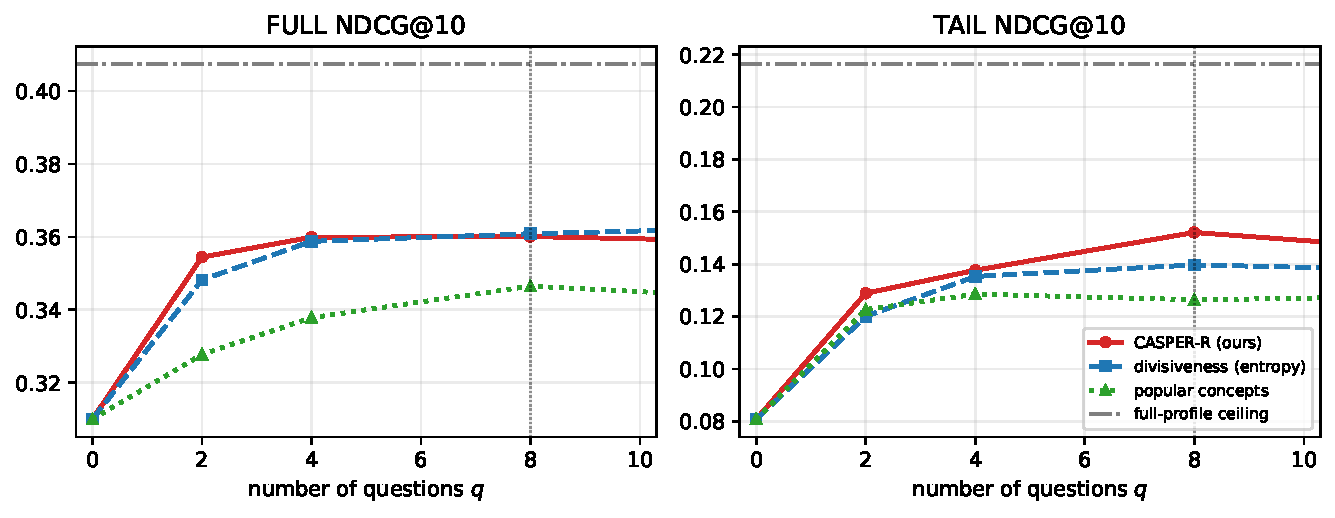
\includegraphics[width=0.94\linewidth]{figs/qcurve.pdf}
\caption{NDCG@10 vs.\ question budget (seed-averaged, te$[300{:}]$, out to $q{=}10$; full left, tail right). CASPER-R
climbs to a \emph{peak} at $q{=}8$ then gently declines (the set-encoder fold is non-monotone in the number of answers);
the heuristics are flat and the full-profile ceiling is constant; full NDCG is popularity-saturated for all. CASPER-R
leads through the realistic budget ($q\le8$); beyond it the curves converge. $T{=}8$ is the sweet spot, not an arbitrary
cut-off.}
\label{fig:qcurve}
\end{figure}

\subsection{The answerability ceiling is efficiency, not endpoint}\label{sec:ansceiling}
Answerability is the realizable lever of this paper (\S\ref{sec:answerresults}); this section bounds how much of the
endpoint it can buy, with two diagnostics on the static-divisiveness (entropy) interview (seed-averaged, te$[300{:}]$,
binary answers).

\textbf{A per-user answerability oracle front-loads but does not raise the plateau.} We keep the fixed divisiveness
ranking but \emph{skip} any concept unanswerable for the current user---peeking only at the $\ge 2$-profile-item
answerability criterion, never at the answer---so all eight turns land, versus the baseline's $5.16/8$ answered. The
lift is entirely early: full NDCG $+0.011$ at $q1$ and tail $+0.014$ at $q2$ ($\sim$2--3$\sigma$), decaying to a tie by
$q8$ ($+0.001$ full / $-0.001$ tail). Perfect answerability lets the asker reach the $q4$ plateau about two questions
sooner; it does \emph{not} raise the plateau.

\textbf{Why: the value of an answered question saturates by $\sim$4 answers.} Within-user, the marginal value of the
$k$-th answered question (the paired NDCG difference at the turn where the $k$-th answer first accumulates) collapses
after a handful of answers (Table~\ref{tab:answered_sat}). Performance saturates at $\sim$2--4 answered questions, so at
the baseline's $5.16$ answered the interview is \emph{already} on the eight-answer plateau; converting the $\sim$2.8
wasted turns into answered turns cannot help at $q8$ because the sixth-through-eighth answers are near-worthless under
the fixed-ranking instrument. The binding constraint on the endpoint is the \emph{informativeness} of later questions,
not their answerability.

\begin{table}[h]\centering\small
\begin{tabular}{l c c}
\toprule
$k$-th answered question & full $\Delta$ & tail $\Delta$\\
\midrule
1 & $+0.020$ & $+0.030$\\
2 & $+0.027$ & $+0.023$\\
4 & $+0.007$ & $+0.002$\\
6 & $-0.001$ & $+0.001$\\
8 & $-0.004$ & $+0.001$\\
\bottomrule
\end{tabular}
\caption{\textbf{Marginal value of the $k$-th answered question} (within-user paired, static entropy, seed-averaged,
te$[300{:}]$). The lift concentrates in the first $\sim$2--4 answers and is $\le +0.001$ tail (and $\approx 0$ or
negative full) from the sixth answer on---so the baseline's $5.16$ answered turns already sit on the plateau.}
\label{tab:answered_sat}
\end{table}

\textbf{A pre-registered anytime-reward test: the front-loading nets to zero.} The one reward recipe with a
training-seed-robust win elsewhere in this project is a \emph{mean-NDCG-over-turns} (``anytime'') reward. We ported it to
the closed-concept harness under a gate frozen before any run: success required a positive tail-NDCG AUC over turns
$1$--$8$ for \emph{all three} training seeds \emph{and} a pooled paired per-user bootstrap $p<0.05$. The result is a
statistical zero. The first (and historically most favourable) training seed gives $\Delta\text{AUC(tail)}=+0.0003$
(paired bootstrap $95\%$ CI $[-0.004,+0.005]$, $p=0.85$), with the secondary metric (tail@$q4$) negative; the gate's
significance arm was therefore unreachable and the campaign was stopped per its no-iteration clause. The mechanism is the
answerability$\leftrightarrow$informativeness tension made concrete: the anytime reward does exactly what it pays for,
raising the answered-question count from $5.16$ to $6.50/8$ by asking more-\emph{answerable} concepts, and converting
that into genuine front-loading (tail $+0.006$ to $+0.010$ at $q1$--$q3$, matching the answerability-oracle headroom
above); but per the saturation curve the answerable-but-less-divisive concepts it substitutes cost late-turn
informativeness (tail $-0.003$ to $-0.008$ at $q4$--$q8$), and the early gain and late loss cancel. A \emph{learned}
policy thus realizes the efficiency bound and no more---even on the AUC yardstick chosen to be maximally favourable to
front-loading. This is why we claim no learned \emph{endpoint} win in the closed-concept setting: the realizable lever
is answerability, its ceiling is early-turn efficiency, and a policy that chases it matches the static heuristic at the
budget's end.

\section{Limitations and outlook}\label{sec:limits}
Our central scoping result---that \emph{learning} or \emph{per-user adapting} the selection adds nothing over a static
one-step surrogate---holds \emph{under the noiseless graded/binary geometric answers} used by our simulator (and by the
conversational-RS simulators we compare against). That regime is close to linear-Gaussian, and in it the optimal
experimental design is essentially non-adaptive: every user answers truthfully, every answerable question lands, and the
belief update is a clean fold. Three deployment nonlinearities break exactly these assumptions, and are precisely where
adaptive value should re-emerge. \emph{(i) Answer noise:} real users answer carelessly or inconsistently, so an answer's
information content becomes state-dependent, and a policy that senses low-confidence answers can re-ask or re-route.
\emph{(ii) Refusal events:} a user may decline or say ``don't know''---a discrete branch a static schedule cannot
anticipate but an adaptive asker can plan around. \emph{(iii) Heterogeneous per-user answer-rates:} users differ in how
many and which question types they will engage, so the answerable pool---and hence the optimal question order---varies by
user. Each is a nonlinearity that restores headroom for adaptivity that the noiseless regime removes; none is exercised
by the present evaluation. The immediate next step is therefore an \emph{answer-noise ablation}---injecting
careless-answer, refusal, and per-user answer-rate models into the simulator---to test whether the learned and adaptive
policies that here only tie the heuristic separate from it once answers stop being clean.

\begin{thebibliography}{99}\small
\bibitem{blau22} Blau, Bonilla, Chades, Dezfouli. Optimizing Sequential Experimental Design with Deep Reinforcement Learning. ICML 2022.
\bibitem{bakker20} Bakker, van Hoof, Welling. Experimental Design for MRI by Greedy Policy Search. NeurIPS 2020.
\bibitem{gsmrl} Li, Oliva. Active Feature Acquisition with Generative Surrogate Models. ICML 2021.
\bibitem{nocta} Dinh, Oliva. Non-myopic Cost-aware Acquisition (NOCTA). arXiv:2507.12412, 2025.
\bibitem{dad} Foster, Ivanova, Malik, Rainforth. Deep Adaptive Design: Amortizing Sequential Bayesian Experimental Design. ICML 2021.
\bibitem{weihs21} Weihs, Jain, Salvador, Lazebnik, Kembhavi, Schwing. Bridging the Imitation Gap by Adaptive Insubordination. NeurIPS 2021.
\bibitem{wolp} Dulac-Arnold et al. Deep Reinforcement Learning in Large Discrete Action Spaces. arXiv:1512.07679, 2015.
\bibitem{conts} Li, Lei, Wu, He, Jiang, Chua. Seamlessly Unifying Attributes and Items: Conversational Recommendation for Cold-Start Users (ConTS). ACM TOIS 2021.
\bibitem{rashid} Rashid, Albert, Cosley, Lam, McNee, Konstan, Riedl. Getting to Know You: Learning New User Preferences in Recommender Systems. IUI 2002.
\bibitem{helf08} Rashid, Karypis, Riedl. Learning Preferences of New Users in Recommender Systems: An Information-Theoretic Approach. SIGKDD Explorations 2008.
\bibitem{golbandi11} Golbandi, Koren, Lempel. Adaptive Bootstrapping of Recommender Systems Using Decision Trees. WSDM 2011.
\bibitem{elahi16} Elahi, Ricci, Rubens. A Survey of Active Learning in Collaborative Filtering Recommender Systems. Computer Science Review, 2016.
\bibitem{ear} Lei, He, Miao, Wu, Hong, Kan, Chua. Estimation--Action--Reflection: Towards Deep Interaction Between Conversational and Recommender Systems (EAR). WSDM 2020.
\bibitem{unicorn} Deng, Li, Zhang, Lei, Huang, He, Chua. Unified Conversational Recommendation Policy Learning via Graph-based Reinforcement Learning (UNICORN). SIGIR 2021.
\bibitem{nicf} Zou, Chen, Chen, Yang, Ye, Du, Zha. Neural Interactive Collaborative Filtering (NICF). SIGIR 2020.
\bibitem{cremonesi10} Cremonesi, Koren, Turrin. Performance of Recommender Algorithms on Top-N Recommendation Tasks. RecSys 2010.
\bibitem{ross11} Ross, Gordon, Bagnell. A Reduction of Imitation Learning and Structured Prediction to No-Regret Online Learning (DAgger). AISTATS 2011.
\bibitem{ng99} Ng, Harada, Russell. Policy Invariance Under Reward Transformations: Theory and Application to Reward Shaping. ICML 1999.
\end{thebibliography}
\end{document}
